\section{ENTRADAS}

El arrecife es especificado desde una archivo de texto plano, donde se encuentran especificadas con n\'umeros (Tiburones, Rocas, Tortugas, Hombres con arp\'on y Metas), seg\'un la especificaci\'on realizada por el Ing. Carlos Delgado y como se muestra en la figura \ref{fig:entrada}
\begin{figure}[!h]
	\centering
	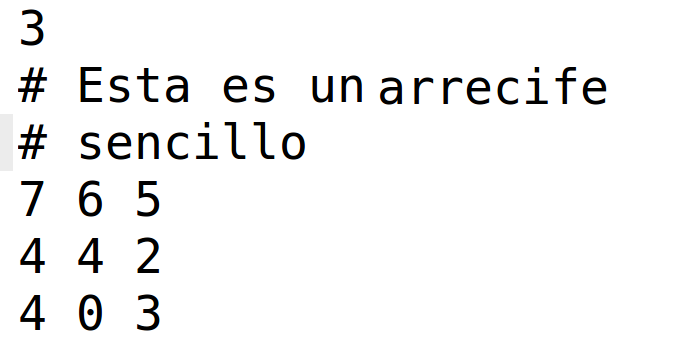
\includegraphics[width=0.25\textwidth]{entrada.png}
	\caption{Entrada simple 3x3}
	\label{fig:entrada}
\end{figure}

Con la finalidad de hacer r\'apida la ejecuci\'on de la aplicaci\'on un archivo es le\'ido una sola vez y en esta lectura se construyen colecciones para cada uno de los elementos del arrecife, una colecci\'on de coordenadas donde se ubican los tiburones, una colecci\'on de coordenadas donde se ubican los obst\'aculos o rocas, etc.

El escenario que se encuentra en memoria puede ser le\'ido por diversos algoritmos, dado que estos obtienen la posici\'on del robot y a partir de este recorre y construye \textit{el grafo}.\\

\textbf{Nemo3} Permite entradas que van desde el 2x2 hasta 20x20, aunque la ejecuci\'on de los algoritmos, tardan mucho tiempo entre mayor sea el escenario y menor cantidad de elementos (Tiburones, Rocas, Tortugas, Hombres con arp\'on y Metas) posea. Un ejemplo de esta situaci\'on es la que indica en las Figuras \ref{fig:areas} una exploraci\'on en las primeras dos figuras podr\'ia costar lo mismo, mientras una exploraci\'on en la gr\'afica podr\'ia tardar un poco mas, claro que esto depende tambi\'en de la estrategia y de condiciones de procesamiento y memoria de sistema en que se ejecuten.
\begin{figure}[!h]
	\centering
	\subfloat[Entrada 8x8 con 64 espacios disponibles]{{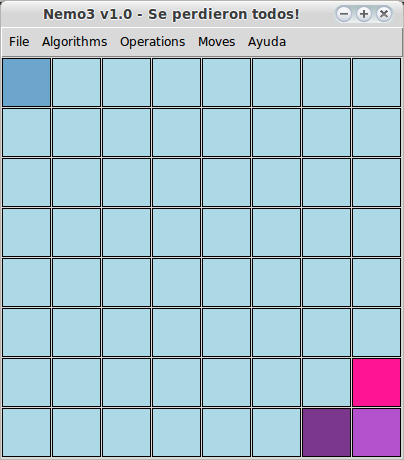
\includegraphics[width=0.2\textwidth]{en8x8.png}}}%
%	\caption{}
	\qquad
	\subfloat[Entrada 12x12 con 64 espacios disponibles]{{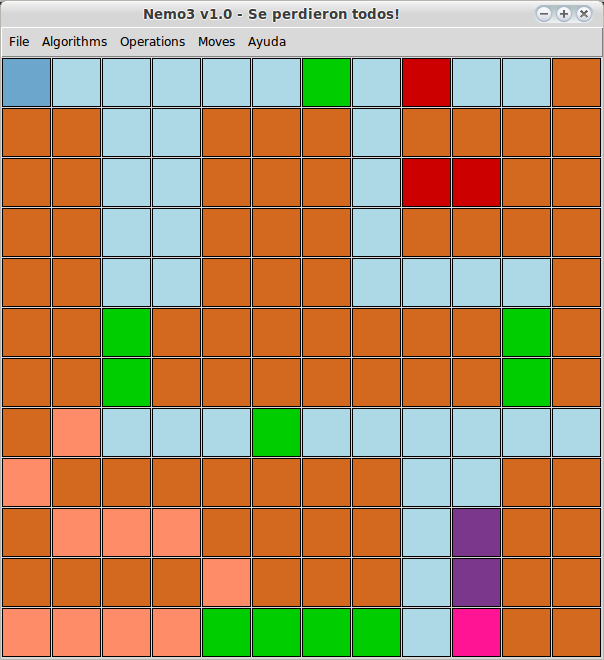
\includegraphics[width=0.2\textwidth]{en10x10.png}}}%
%	\caption{}
%	\qquad
%	\subfloat[entrada 2x2 con tres soluciones]{{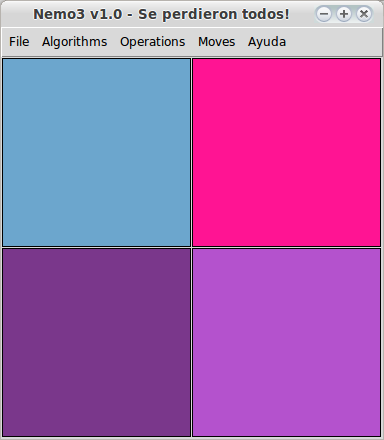
\includegraphics[width=0.1\textwidth]{en2x2.png}}}%
%	\caption{En las primeras dos gr\a'aficas el tiempo y la amplitud para un mismo algoritmo podr\'ia tardar lo mismo por el tama\~no de la exploraci\'on.\\En la entrada 2x2 la exploraci\'on deber\'ia ser menor}
	\label{fig:areas}
\end{figure}

Esto sera ampliado en la discusi\'on y el an\'alisis de los resultados. Algunas de las pruebas de entrada fueron creadas a partir de un generador ASCII en linea, con diversas dimensiones.